\chapter{Introduction\label{chap:introduction}}
\section{Overview}
% Drug discovery is important. 
Drug discovery is the process of identifying new medicines and bringing them to
market. The discovery of novel pharmaceutical treatments has been a major driver
of quality of life over the centuries. While discovery of new drugs has started 
in serendipitous and lucky discoveries, advances in science and technology  
led to an ever more systematic and data-driven approach, especially over the
last decades. 

% The process is hard and expensive
Finding a new drug is a highly complex, expensive and time-consuming endeavor. 
The estimated costs of drug discovery projects range from x-y \citep{todo} 
and take up to x years \citep{todo}. 

% Computer aided drug discovery
Computer aided drug discovery (CADD) aims to accelerate the drug discovery
process using computational methods. Applications range from basic chemical
information processing, over physical simulation of molecular interactions, to
sophisticated machine learning methods. Recently, advances in deep learning
have led to breakthroughs in many different
areas of drug discovery \citep{chenRiseDeepLearning2018}, including highly accurate protein structure prediction 
achieved by AlphaFold \citep{todo}, chemical property prediction
\citep{mayrDeepToxToxicityPrediction2016,todo}, synthesis planning
\citep{seglerNeuralSymbolicMachineLearning2017} and molecule generation
\citep{todo}. These advances help by reducing the need for expensive 
wet-lab experiments and can assist chemists in drug design tasks. 

% Significance and objectives of the thesis
In this thesis we focus on generative models for molecules. Generative models
are a class of machine learning models that generate molecular structures
relevant to a given task. However, the evaluation of generative models is
challenging, as the outputs of these models are usually complex, structured
objects, and there are often no straightforward ways to evaluate the quality or
relevance of the generated molecules. In this thesis, we address this issue by
proposing new evaluation metrics and benchmarks for generative models.

% Synthesis planning
We also study the application of generative models to computer-aided synthesis
planning (CASP). CASP tools assist chemists in the task of synthesizing target
molecules. These tools rely on retrosynthesis prediction models, which predict
the reactants that can be used to synthesize a target molecule. We propose a
novel retrosynthesis prediction model that improves the generalization capabilities 
of template-based models. We also propose new evaluation metrics and highlight
trade-offs between accuracy and throughput in retrosynthesis prediction.

% PROMISE
This thesis is structured as follows. In \cref{sec:drug-design} we give an
overview of small molecule drug design, the drug discovery pipeline 
and how computer aided drug discovery can help to accelerate this process.
In \cref{sec:generative-models} we give an overview of generative models for
molecules and discuss the challenges of evaluating these models In \cref{sec:retrosynthesis} 
we give a short overview of computer-aided synthesis planning.
\Cref{sec:retrosynthesis} gives an overview of retrosynthesis prediction and
the associated challenges. \Cref{sec:aims-objectives} gives an overview of the
aims and objectives of this thesis. \Cref{sec:publications} lists the publications 
that are part of this thesis and related publications. 
\Cref{chap:publications} reprints the publications and
their corresponding supplementary material. Finally, \Cref{chap:conclusion}
concludes the thesis and gives an outlook on future work.



% \begin{minipage}
% : Rational drug discovery.
% This approach starts with the identification of a biological target in the body 
% which is hypothesized to be associated with a disease phenotype. 
% One then attempts to find a small molecule that can change the activity of 
% the target in the desired way. While this way of searching for new drugs 
% is more direct than phenotypic drug discovery the identification of 
% drug targets can be challenging and given the complex interconnectedness 
% of biochemical pathways, it is not fully understood how some drugs work, 
% which goes even for highly popular ones.

% Phenotypic drug discovery takes this trial-and-error approach and applies it 
% in a systematic manner. The focus in this approach, which is also called forward 
% pharmacology, lies on screening collections of small molecules or other potential 
% medicines for pharmaceutical effects. Once a pharmacologically active molecule 
% has been found the aim is to discover how to use it's effect therapeutically. 
% This process can proceed without knowing the biochemical mode of action, of how 
% a drug actually achieves its effect. 

% How were new medicines discovered?
% David C. Swinney & Jason Anthony 
% Lots of molecules also by phenotypic screening

% One of core goals in both approaches is to find molecules with a desired
% pharmacological profile, which includes primarily the ability of a molecule to
% modify a target, but also other important
% properties, e.g. absorption, distribution, metabolism, excretion or toxicity. 
% To find such molecules, specially designed wet-lab experiments called \emph{assays} 
% are usually use to measure these properties of interest. The number of tested 
% molecules can range from numbers in the tens to millions of tested molecules
% in high-througput screening. 

% \emph{Computer-aided drug design} aims to reduce the need 
% for these expensive experiments using computational methods. 
% The field of quantitative structure activity/property relationship (QSAR/QSPR)
% aims to find an accurate computational model of the drug-target interaction. 
% Structure-based methods make use of the known structures of the drug and target 
% and calculate binding affinity using physical modelling. 
% In contrast, ligand-based methods find links between molecular structures
% and measured experimental outcomes. In recent years, machine learning methods 
% have shown great promise at modelling these relationships. 
% Using these models one can prioritize which of the molecules available in a screening 
% collection to test next, to avoid wasting ressources on unpromising compounds.

% However, this approach of virtual screening is limited to existing screening collections
% and computational constraints. The $~10^{12}$ \citep{todo} molecules that can be realistically 
% evaluated fall far short of the $10^{23}$-$10^{60}$ drug-like molecules 
% which are estimated to exist \citep{todo}, and necessarily miss out on promising drug candidates.
% Generative models aim to alleviate this problem, by using the QSAR/QSPR function as a guiding signal 
% in order to be able to explore chemical space in a goal-directed manner. 
% The evaluation 

% However, the process of bringing a new drug to market is a long, expensive, and risky endeavor.
% Estimates of bringing a new drug to market range between 2.6 and xxx 
% billion USD \citep{todo}. When successful, however, a new drug can be a major source of
% relief for patients.

% % Traditional way of finding candidates.
% One of the key challenges of the drug discovery process is the identification
% of novel promising drug candidates. Traditionally, this is done by synthesizing
% and testing the molecules efficacy in a laboratory and clinical studies. 
% However, this process is usually very expensive, time-consuming and can be risky for 
% patients. 

% % ML can help to find promising candidates
% Machine learning (ML) and deep learning (DL) have the potential to accelerate
% the drug discovery process. Recent advances in ML, especially in the subfield of deep learning
% have led to a surge in interest in applying ML and DL to drug discovery, 
% culminating in breakthroughs such as AlphaFold \citep{todo}. 
% In this thesis, we focus on two key areas where ML and DL can help to accelerate
% the drug discovery process: generative models for molecules and computer-aided
% synthesis planning (CASP).
% \end{minipage}

\section{Small molecule drug design\label{sec:drug-design}}
\subsection{Requirements for small molecule drugs\label{sec:requirements}}
Small molecule drugs are the major kind of medicines in use, with as much as
90\% of global sales \citep{makurvetBiologicsVsSmall2021}.
For a small molecule to be a viable drug candidate it needs to fulfill a whole range 
of properties \citep{todo}:
\begin{itemize}
    \item \textbf{On-target activity:} The molecule needs to be active against
    the desired target in order for it to show the desired therapeutic effect.
    On a molecular level this means that the molecule needs to bind to the target
    and modulate its activity in the desired way. 
    \item \textbf{Pharmacokinetics:} The molecule must have favourable
    pharmacokinetic properties such as adsorption, distribution, metabolism and
    excretion (ADME). ADME determine how the molecule is absorbed into the
    body, how it is distributed in the body, how it is metabolized and how it is
    excreted from the body. These properties are crucial for the molecule to
    reach the target in the body and to be metabolized in a safe manner and to 
    finally be excreted from the body.
    \item \textbf{Toxicity:}  The absence of toxic effects is crucial, as the
    molecule must be well-tolerated and devoid of any potential harmful side
    effects. Toxicity can be caused by a range of factors, including off-target
    interactions, metabolic byproducts or allergies.
    \item \textbf{Specificity:}  The molecule should exhibit high specificity,
    selectively interacting with the intended target while minimizing
    undesirable off-target interactions. Off-target binding can lead to adverse
    side effects and potentially compromise the drug's safety and efficacy
    profile.
    \item \textbf{Synthesis:} The molecule must be synthesizable in a
    cost-effective manner to be practically useful.
    \item \textbf{Patentability:} The molecule must be novel and not infringe on
    any existing patents. While in general this is not needed for a drug to work, 
    this constitutes a significant issue in practice.
\end{itemize}

\subsection{The Drug Discovery Pipeline}
% Drug discovery is complex and expensive. 
The process of discovering a new drug is a complex and multi-faceted task. The
cost of bringing a new drug to market is estimated to be between 2.6 and 3.0
billion USD \citep{todo} and the process can take up to 10-15 years
\citep{todo}. The process is usually structured into multiple stages,
leading from the initial identification of a biological target to the final
approval of the drug by regulatory agencies. The core idea is to start 
with many potential drug candidates and to systematically reduce this number
to a few promising candidates that can be tested in clinical trials.
Throughout this process, the properties of the molecules are tested in a
variety experiments, that get more and more complex and expensive (per compound) as the
process progresses. \Cref{fig:drug-discovery-pipeline} gives an overview of the
drug discovery pipeline and we will discuss the stages in more detail next:

\begin{figure}
    \centering
    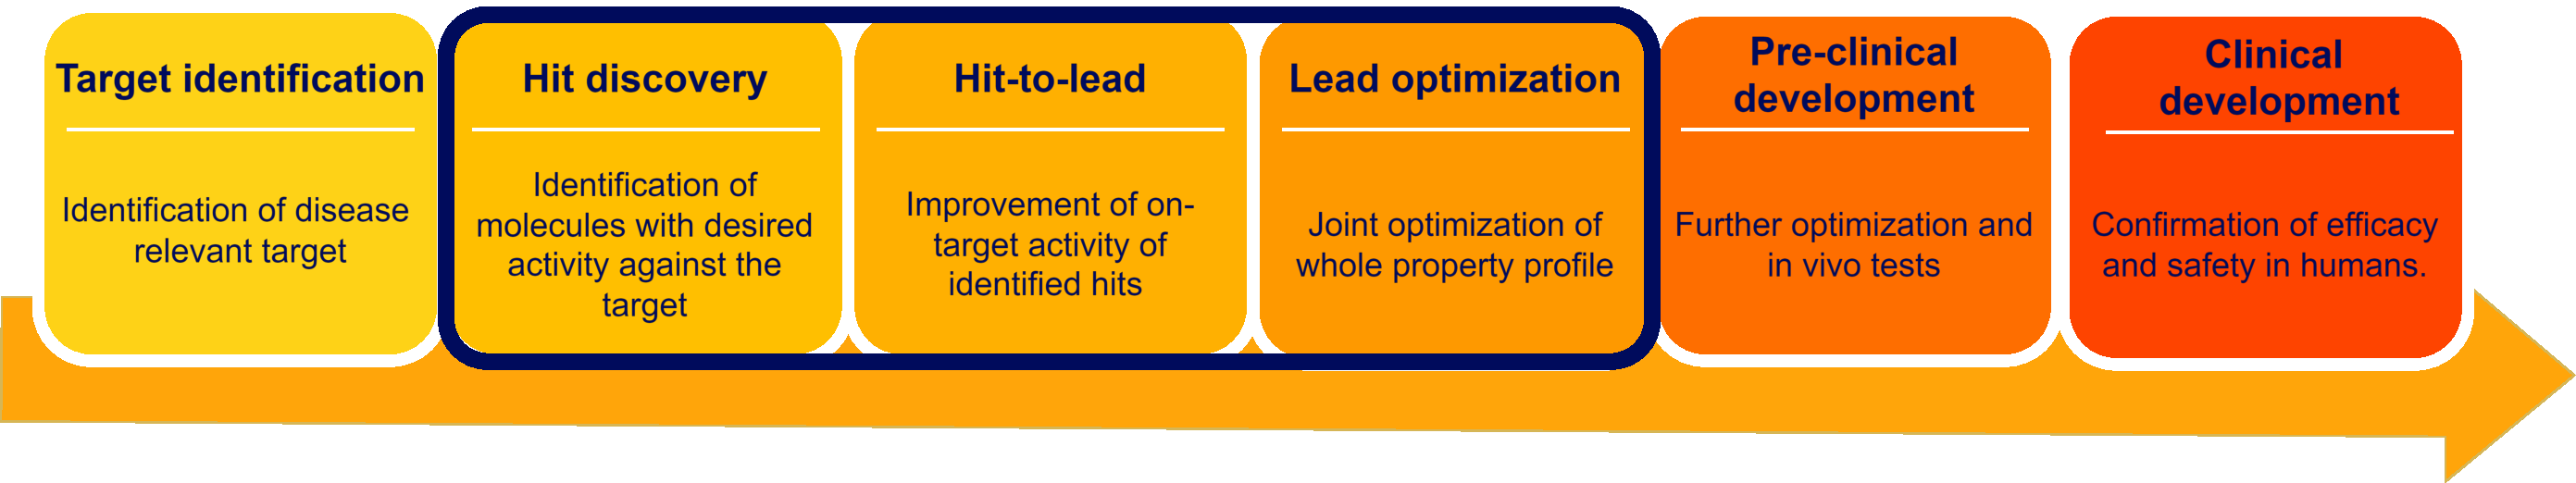
\includegraphics[width=\textwidth]{figures/drug-discovery-pipeline.pdf}
    \caption{The drug discovery pipeline starts with the identification of a
    biological target. Once a target is identified, readily available molecules
    are screened for their activity against the target in high-throughput
    screening. Promising hits are then modified and optimized to lead compounds.
    These lead compounds are then further optimized and tested in preclinical.
    Finally, the most promising candidates are tested in clinical trials and
    eventually approved by regulatory agencies. The stages in the blue box are
    highly amenable to machine learning and computational methods and are the
    focus of this thesis. \label{fig:drug-discovery-pipeline}}
\end{figure}
\begin{itemize}
    \item \textbf{Target identification:} The first stage is target identification, 
    where a biological target is identified that is hypothesized to be associated
    with a disease phenotype.
    \item \textbf{Hit discovery:} In the hit discovery stage molecules are
    screened for their activity against the target in high-throughput screening (HTS).
    These lab experiments ,often referred to as assays, are used to measure the
    activity of the molecules against the target in vitro. HTS is resource
    intensive and time-consuming.
    \item \textbf{Hit-to-lead:} Promising hits are then modified and optimized
    to lead compounds. In this stage, the optimization is primarily focused on
    improving the activity of the molecule against the target. This is usually 
    done in a DMTA (Design-Make-Test-Analyze) cycle, where the molecule is
    designed, synthesized, tested in vitro. The results are then analyzed and the cycle 
    continues until a satisfactory lead compound is found.
    \item \textbf{Lead optimization:} The lead compounds are then further
    optimized to improve their properties, such as pharmacokinetics, toxicity or
    specificity. This is usually done in a DMTA cycle as in the
    hit-to-lead stage and also involves the synthesis and testing of the
    molecules in vitro.
    \item \textbf{Preclinical development:} The most promising candidates are then tested in
    preclinical studies. These studies are usually done in animals and are used
    to assess the safety and efficacy of the drug candidate in vivo. 
    \item \textbf{Clinical trials:} Finally, the candidates that pass the
    preclinical studies are tested in humans in clinical trials. 
    These are usually divided into three phases, where the safety and efficacy
    of the drug are tested in increasing numbers of patients. 
    Phase I trials are mainly focused on the safety of the drug, Phase II trials
    are focused on the efficacy of the drug and Phase III trials are focused on
    the safety and efficacy of the drug in a larger population.
    \item \textbf{Regulatory approval:} The final stage is the regulatory
    approval, where the drug is approved by regulatory agencies such as the FDA
    in the US or the EMA in Europe. 
\end{itemize}

% The chances of success are low
The success rates of clinical trials are low, with only about 10\% of drugs that
enter clinical trials eventually being approved by regulatory agencies
More specifically, the success rates in Phase I/II/III and the final 
regulatory approval are 63\%, 31\%, 58\% and 85\% respectively 
\citep{mullardParsingClinicalSuccess2016}. This translates to
63\%, 19.5\%, 11.3\% and 9.6\% of projects that make it to the respective stages
\citep{mullardParsingClinicalSuccess2016}. 

The final answer whether a molecule represents a useful drug only comes from
testing it in clinical trials. As these are expensive and risky, the goal of the
preceeding preclinical stage is to approximate the outcome of the clinical
trials as closely as possible. This applies recursively to the stages before,
where the goal is to approximate the outcome of the next stage as closely as
possible at a lower cost. 

Multiple molecules are usually passed from stage to stage, with the number of
molecules decreasing with the progress of the pipeline. 
In the hit discovery stage, it is possible to test large numbers of 
compounds and pass the most promising ones to the hit-to-lead stage.
It is important to pass on diverse sets of promising molecules, as 
the chances are low that any single molecule will be successful.
Testing similar molecules is usually not useful, as the results are 
usually correlated and the information gain does not justify the
cost of the experiment. A diverse set of molecules is more likely to
contain a successful candidate.

Overall the drug discovery pipeline starts out with a large number 
of molecules where there is high uncertainty about their usefulness.
As the pipeline progresses, the number of molecules decreases and
the uncertainty decreases, until the final stage
where the molecule is tested in clinical trials and the uncertainty
is at its lowest.

The hit discovery, hit-to-lead and lead optimization (blue box in
\Cref{fig:drug-discovery-pipeline}) are highly amenable to machine learning and
computational methods and are the focus of this thesis. Specifically 
we will focus on generative models for molecules, which can help to 
find hits in the hit discovery stage and optimize lead compounds in the
hit-to-lead and lead optimization stages. Furthermore we will look at 
computer-aided synthesis planning (CASP) tools, which can help to find
synthesis routes for promising molecules in the hit discovery, hit-to-lead and lead optimization
stages.

\subsection{The Design-Make-Test-Analyze cycle}
\begin{figure}
    \centering
    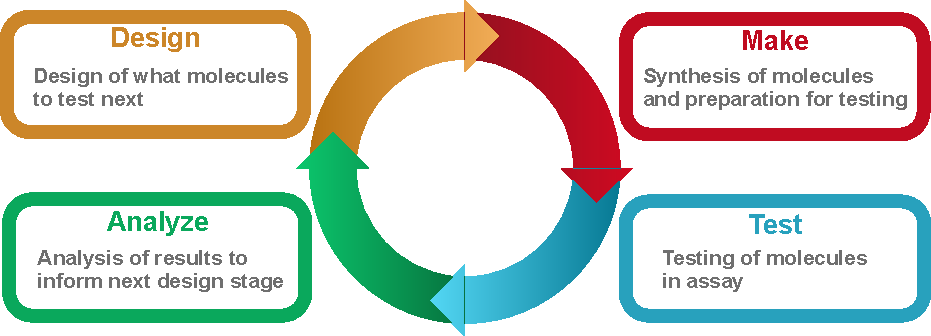
\includegraphics[width=\textwidth]{figures/dmta_cycle.pdf}
    \caption{The DMTA cycle}
\end{figure}
% Drug discovery equals searching chemical space 
Essentially drug discovery can be viewed as the process of searching 
chemical space for medicines. The drug discovery pipeline introduces 
a structured process to navigate this space in a systematic manner, 
that makes the search feasible in the end. Each conducted experiment
has the goal of gathering information and reducing the uncertainty
relating to the molecules under consideration.

% The DMTA cycle
While the stages of the drug discovery pipeline are usually linear, the
precosses within each stage are usually highly iterative. Experiments are
conducted in an iterative manner, where the results of previous experiments are
used to guide the design of the next experiment. This process is usually
referred to as the \ac{DMTA}-cycle:
\begin{itemize}
    \item \textbf{Design:} Design of the molecule to be
    tested. The design is based on previous experimental results and
    aims to maximize the information gain of the next experiment.
    This happens under consideration of the synthesizeability.
    \item \textbf{Make:} The molecules are then synthesized in the laboratory
    and prepared for testing.
    \item \textbf{Test:} The synthesized molecules are then tested in
    laboratory experiments to measure the properties of interest.
    \item \textbf{Analyze:} The results of the experiments are then analyzed
    and used to guide the design of the next molecule to be tested.
\end{itemize}

% \begin{itemize}
%     \item \textbf{Proxy models:} One way is to use proxies, which 
%     aim at approximating the outcome of an expensive experiment at a lower cost.
%     Conducting a clinical trial is very costly and it would be impractical (and unethical) to
%     test a drug candidate without prior testing in vitro and in animals. 
%     In practice multiple layers of varying complexity are used ranging 
%     from animal studies over in vitro assays to in silico methods.
%     \item \textbf{Incorporting experimental feedback:} The second strategy
%     involves selecting future molecules for testing based on previous
%     experimental results. For example, ressources should not be wasted on
%     molecules that are very similar to ones already found undesirable. While
%     this may seem straightforward, it requires a certain level of sophistication
%     and intelligence in the decision-making process.
% \end{itemize}


\subsection{Computer-Aided Drug Design}
\Ac{CADD} aims to accelerate the drug discovery
process using computational methods, offering support throughout all stages of 
the drug discovery pipeline and all steps of the DMTA cycle.
The are three major ways CADD can be of help in the DMTA cycle.

\subsubsection{Molecular property prediction}
\Ac{QSPR} models are used to predict properties of a molecule given 
its structure. Important properties to be modelled are the ones listed in \ref{sec:requirements}, 
but the list also includes others. For example, physico-chemical properties like molecular weight,
water-octanol partition coefficient (logP). 
One of the core tasks is the prediction of activity of a molecule against a biological target. 
This is usually referred to as \ac{QSAR} modelling. These models can be grouped into 
structure-based and ligand-based methods.

Structure-based methods use the known structure of the protein target and determine the interaction 
between a molecule and the target using a physical model. 
This does not come without challenges. The accuracy of these models is often lacking and the simulations 
often have high computational cost. These methods have received increased attention 
after AlphaFold \citep{todo} has significantly improved protein structure prediction.

Ligand-based methods learn a model of molecular activity using activity values obtained in experiments.
\newcommand{\reals}{\mathbb{R}}
These models rely on a set of activity measurements $\{(x_1, y_1), \dots, (x_n, y_n)\}$, where $y_i \in \reals$ is the measured 
activity for a molecule $x_i$. Ligand based methods then train \ac{ML} methods to find a function with high 
predictive performance. In recent years, this approach has seen lots of progress mainly  due to the 
development of novel \ac{DL} methods \citep{todo}. While showing good performance, this approach 
can have problems when little or no data is available. 
% Add that models fitted and evaluated is done in analyze stage.

\subsubsection{Virtual Screening \& De Novo Drug Design}
\begin{figure}
    \centering
    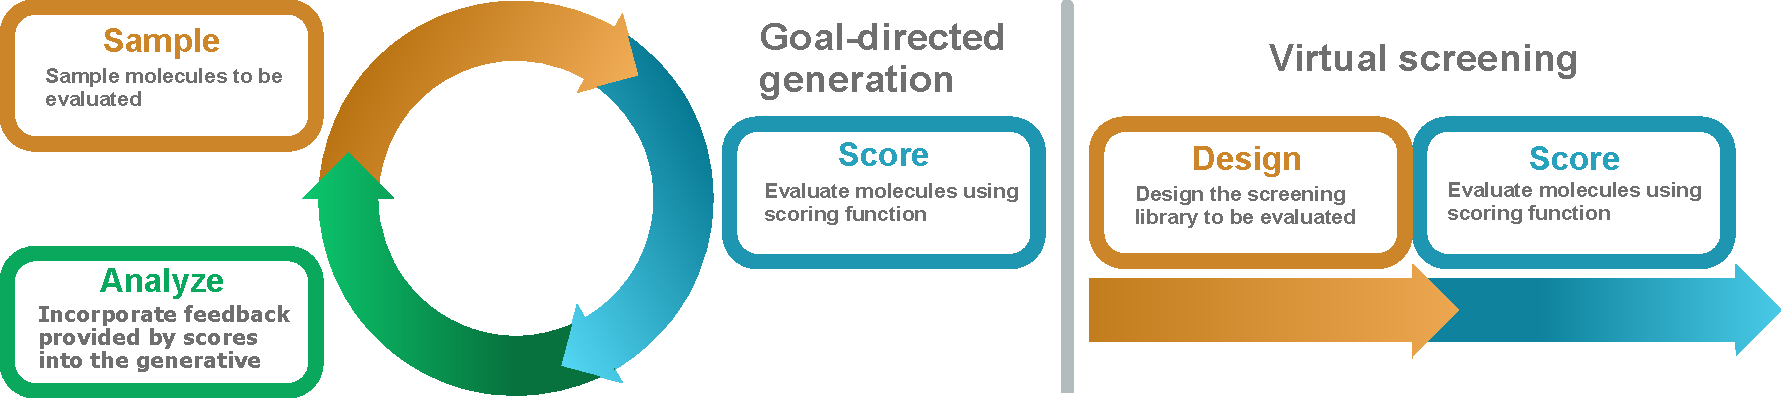
\includegraphics[width=\textwidth]{./figures/goal_directed_cycle_and_virtual_screening.pdf}
    \caption{Comparison of goal-directed generative models and virtual screening.
    Goal-directed generation proceeds in a loop where already scored molecules 
    inform what molecules to test next. Virtual screening proceeds in a linear 
    fashion, where the molecules to be tested are determined beforehand. 
    }
\end{figure}
The \ac{QSPR} models introduced in the previous section can then be used during
the design phase of the DMTA cycle. When designing the next batch of molecules to be made and tested
the properties of the draft molecules are predicting and unpromising compounds can be discarded. 
This reduces the synthesis and testing costs. While these methods can be of help to chemists 
manually designing molecules, they are most prominently applied in automatic selection 
of molecules. For this there are two main approaches: \Ac{VS} and \ac{DNDD}

% What is it for?
\Ac{VS} searches for promising molecules by ranking a given set of molecules according 
to their predicted properties. The set of molecules is usually referred to as a screening library.
Screening libraries can be based on a variety of sources. A popular choice is the set of compounds 
that can be ordered from commercial vendors or are already in stock. These libraries are limited 
in size however \citep{todo}. Combinatorial libraries such as \citep{todo} offer a bigger range of 
molecules that can be synthesized with high probability.
% These libraries can for example be 
% based on virtual combinatorial chemistry, where molecules are generated
% by combining fragments of molecules using chemical reaction rules. 




% Limitations
While \ac{VS} methods have been successful in improving 
the fraction of molecules that are successfully tested, they have limitations. 
Naturally they the outputs of a \ac{VS} run can only be as good as the
underlying prediction model. A second limitation is that \ac{VS} methods
usually do not make use of the feedback of already tested molecules.
Instead, they scan the library of molecules in random order, which 
can make the search inefficient, as ressources are wasted on molecules
that are very similar to ones already found undesirable.
This is especially problematic for prediction models that are 
computationally expensive to evaluate. 

% This chemical space, which encompasses all possible drug-like
% molecules that could be synthesized, is immense, with estimates ranging from
% $10^{23}$-$10^{60}$ potential molecules \citep{todo}. Navigating this space
% effectively and efficiently is a critical challenge in medicinal chemistry and
% pharmacology. 


\subsubsection{De-novo drug design}
\Ac{DNDD} aims to design new molecules with desired properties from scratch.
\Ac{DNDD} is also based on \ac{QSPR} models, which are used to guide the
design of new molecules. These models can be used to generate new molecules
from scratch or to modify existing molecules to improve their properties.
It forms an alternative to \ac{VS}, with the hope of being able to search
chemical space more efficiently. \ac{DNDD} relies on generative models, 
which are able to generate molecular structures relevant to a given task.

In recent years, there has been a resurgence of interest in generative models,
triggered by advances in \ac{DL}. \ac{DL} models have shown great promise in
processing complex, structured data, such as images and text \citep{todo}.
Inspired by these successes, researchers started adopting \ac{DL} models for 
drug discovery. These were particularly helpful in the domain of generative
modeling.



% In the context of computer-aided drug discovery (CADD), the use of proxy
% models translates to the use of quantitative structure-activity relationship
% (QSAR) models, which predict molecular properties of interest, such as the
% activity of a molecule against a target, its pharmacokinetic properties or its
% toxicity. 
% These two strategies can be combined at every stage of the drug discovery process.
% Batched high-throughput screening (HTS) is an example of a routine
% that uses both of these strategies. In this routine, a batch of molecules is
% tested in a single experiment. The results of this experiment can 
% then be used to plan the next batch of molecules to be tested using 
% a machine learning model as a cheaper proxy. This model predicts the
% outcome of the more expensive wet-lab experiment, and can 
% discard unpromising molecules before they are tested.
% However, virtual screening itself does not make use of the feedback 
% of already tested molecules itself. Instead, it searches chemical 
% space in a brute-force manner, by evaluating a fixed library of molecules
% in order. 

% Generative models aim at addressing this gap by incorporating the 
% feedback of already tested molecules into the search process.
% By using the results of already scored molecules as a guiding signal, 
% generative models offer the hope of being able to search chemical space
% more efficiently. While in later stages of the drug discovery pipeline 
% medicinal chemists can use their intuition and experience to guide the
% search, in the early stages of the pipeline, where the number of molecules
% under consideration is large, generative models take over the role 
% of designing the next molecule to be tested.


\section{Generative Models in Drug Discovery\label{sec:generative-models}}
% Generative model introduction 
Generative models are a class of machine learning models that 
generate new data samples. This is in contrast to classification/regression models,
which predict a label or a continuous value for a given input. 
In the context of small molecule drug design, generative models may be 
used to generate molecules with desired properties or to solve 
other tasks such as synthesis planning. 

In this section we will give an overview of generative models for molecules.
We start with different ways to represent molecules and then discuss 
different approaches to generate molecules. We will then give an overview 
of three important generative modelling tasks in drug discovery:
de novo drug design and computer-aided synthesis planning.

\subsection{Molecular Representations}
\begin{figure}
    \centering
    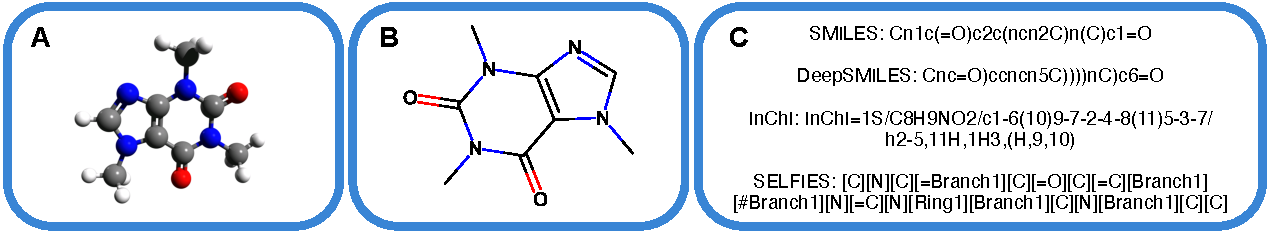
\includegraphics[width=\textwidth]{figures/representations/representations.pdf}
    \caption{Different ways to represent molecules. The molecule shown 
    is caffeine \textbf{A:} Different 1D representations of a molecule. SMILES is an established 
    line notation for molecules. DeepSmiles enables easier generation of
    molecules by getting rid of pair brackets and ring numbers. SELFIES
    guarantees that a sequence of tokens parses into a valid molecule.
    \textbf{B:} 2D graph representation of a molecule. The nodes represent
    atoms and the edges represent bonds. 
    \textbf{C:} 3D structure of a molecule. The atoms are positioned in 3D
    space. The positions of these atoms can change as some bonds are 
    allow rotations. Source of the 3D structure: \citep{EnglishCaffeine3D2010}.
    \label{fig:molecular-graph}}
    % TODO: add adjacency matrix representation
\end{figure}
Molecules are complex objects that can be represented in a variety of ways.
While molecules are complex quantum mechanical objects, there exist 
a variety of more simple, practically useful representations of molecules.
Molecules are formed by atoms, which are connected by chemical bonds.
The connectivity between the atoms can be represented as a graph, where
the nodes represent atoms and the edges represent bonds. Additionally,
the atoms/bonds by their atom/bond type and other properties such as
charge or chirality. This representation is called a molecular graph.

Molecules can also be represented as a 3D structure, where the atoms are
positioned in 3D space. This representation is useful for studying the
interactions of molecules with other molecules or proteins. 

Molecular graphs can also be linearized into a 1D sequence of characters. Line
notations such as INCHI \citep{todo} or Simplified Molecular Input Line Entry
System (SMILES) \citep{weiningerSMILESChemicalLanguage1988} represent molecules
as 1D representations of characters. SMILES strings have turned out to be a
highly useful representation of molecules in the context of generative models,
as they are easily processed by sequence-based models such as recurrent neural
networks (RNNs) or transformers \citep{vaswaniAttentionAllYou2017}. Several
extensions for this molecular representation have been proposed, such as SELFIES
\citep{krennSELFIESFutureMolecular2022}, DeepSmiles
\citep{oboyleDeepSMILESAdaptationSMILES2018} or SAFE
\citep{noutahiGottaBeSAFE2023}. 

\subsection{Generative modelling approaches}
There is a wide variety of approaches to generate molecules. These approaches
differ in the way they represent molecules, the way they generate molecules
and the way they are trained. In the following we will give an overview of
some of the most popular approaches to generate molecules. 

\subsubsection{Assembly strategies}
\paragraph{Autoregressive models} constitute one of the most popular approaches
to generative models for generating discrete 1D/2D molecular representations. 
These models start with an "empty" molecule and iteratively add to it. 
At each step, the model takes the current state of the molecule chooses 
a modification to apply from a set of possible modifications. This modification
is then applied to the molecule and the process is repeated until a special
end-of-sequence action is taken. Mathematically this can be formulated as
\begin{align}
    p(x) = \prod_{i=0}^n p(x_i | x_{0:i-1}), 
\end{align}
where $x$ is the molecule and $x_i$ corresponds to the state of the molecule 
at step $i$. This gives us a probability distribution over the space of molecules
and to evaluate the likelihood of a given molecule. Models for which this fact 
holds are called explicit density models.

One of the most popular approaches is to use recurrent neural networks (RNNs)
or Transformer models \citep{vaswaniAttentionAllYou2017} model 1D sequences.
These models have been used to generate SMILES, SELFIES or DeepSmiles strings
\citep{seglerGeneratingFocusedMolecule2018,todo}. 
In most cases, the training data is a set of molecules and the model is trained
to maximize the likelihood of the training data. The molecules are usually
tokenized into the grammatical units of the used representation before training. 
The model is then trained to predict the next token in the sequence given the
previous tokens.

Another approach to autoregressive modelling is to use graph-based models, which
model the molecular graph directly. These models are based on graph neural
networks (GNNs) and are used to generate molecular graphs directly. 
These models start with an empty graph and iteratively add nodes and edges to
it. At each step the model chooses a modification to apply to the graph and
applies it. While the specification of possible actions is usually more 
complex than in the 1D case, the model can be trained in a similar manner.

% https://www.frontiersin.org/journals/hematology/articles/10.3389/frhem.2024.1305741/full#h4
\paragraph{Rule-based models} are another approach to generate molecules. These
models are based on graph transformation rules, which are used to generate
molecules. These rules are often manually defined and/or represent 
transformations that represent chemical reactions. 
Notable examples of this approach are: 

\begin{itemize}
    \item Fragment spaces: The BRICS \citep{degenArtCompilingUsing2008} method
    provides a set of molecular fragments and rules how to meaningfully combine
    them. This enables the generation of new molecules by combining these
    fragments.
    \item DOGS \citep{hartenfellerDOGSReactionDrivenNovo2012} provides a 
    set of readily available building blocks and synthetic principles how to 
    combine them. 
    \item \citep{bradshawBarkingRightTree2020,gottipatiLearningNavigateSynthetically2020} formulates a general framework 
    of creating synthesis graphs relying on a chemical reaction model.
    \item \citep{jensenGraphbasedGeneticAlgorithm2019} defines graph mutation 
    and crossover operations to generate new molecules. 
\end{itemize}
These models allow the generation of molecules that are chemically valid, 
or resemble known "reasonable" molecules. While basic properties of 
the generated molecules can be made to resemble a training set, 
these models do not allow more complex training objectives. 

\paragraph{\Acp{VAE}} are another popular approach to
generate molecules. \Acp{VAE} are latent space models, which sample 
data by first sampling from a simple latent distribution $p(z)$, which is often 
a multi-variate normal distribution. The samples are then mapped to 
molecular space via a probabilistic decoder network $p(x|z)$.
To make training tractable a second network, the encoder network $q(z|x)$ is
used to map the data to the latent space. The model is trained to maximize
the evidence lower bound (ELBO) of the data
\begin{align}
    \log p(x) \geq \mathbb{E}_{q(z|x)}[\log p(x|z)] - \text{KL}(q(z|x) || p(z)), 
\end{align}
where KL is the Kullback-Leibler divergence. 
This model has the advantage of providing a continuous latent space, which can
be used to interpolate between molecules or run optimization algorithms in
latent space. Calculating the likelihood of a given molecule is not possible
in this model as it requires the integration over the latent space
\begin{align}
    p(x) = \int p(x|z) p(z) dz,
\end{align}
which is usually intractable. This type of model is called an approximate density model. 

% molgan
\paragraph{Generative adversarial networks (GANs)} are similar to VAEs in that
they also sample from a simple distribution in latent space, $p(z)$ and map the samples to 
molecular space via a generator network $p(x|z)$.
However, the training of GANs is based on a game-theoretic approach, where a
generator network is trained to generate samples that are indistinguishable from
the training data. The training signal is provided by a discriminator network,
which is trained to distinguish between real and generated samples. The generator
is then trained to minimize the discriminator's ability to distinguish between
real and generated samples. GANs have been used to generate molecules 
in a variety of representations \citep{todo}. In general the generator network
is not invertible, which means that the likelihood of a given molecule cannot
be calculated. This makes GANs implicit density models, which define a 
likelihood function $p(x)$ only implicitly via sampling, but not explicitly.

% moflow, graphnvp (has nice discussion on one-shot generation)
\paragraph{Generative flows} are based on the idea of learning a bijective
mapping between the data space and a latent space. These 
models sample molecules by first sampling from a simple distribution in latent
space, $p(z)$ and then mapping the samples to molecular space via a
bijective mapping $G: z \rightarrow x$. The model is trained to maximize the
likelihood of the training data, which can be calculated exactly via 
the change of variables formula:
\begin{align}
    p(x) = p(z) \left| \det \frac{\partial G}{\partial z} \right|.
\end{align}
The mapping $G$ is usually implemented as a neural network, which consists
of a series of invertible transformations, which combined can approximate 
complex transformations. These models were first introduced for continuous data
\citet{rezendeVariationalInferenceNormalizing2016}. The extension to molecules,
which are discrete data, necessitates using a continuous relaxation of the
molecule. This is often done by modelling the adjacency/node feature matrix of
the molecule as a continuous variable. These models also belong to the class of
explicit density models, as the likelihood of a given molecule can be calculated
exactly.

\paragraph{GFlowNets} ...

\paragraph{Rule based models} are another approach to generate molecules. These
models are based on a set of rules, which are used to generate molecules.

\paragraph{Diffusion models} also rely an a variational bound and are approximate
density models.

\paragraph{Alternative approaches} There are a variety of alternative approaches
such as 3d modelling which we will not discuss in detail here.
    
Triggered by advances in deep learning, the field of generative models for
molecules has seen a surge in interest in recent years. The first deep-learning
based generative models for molecules were based on recurrent neural networks
(RNNs) originally proposed for text generation. After this early work by
\citep{seglerGeneratingFocusedMolecule2018} and
\citep{gomez-bombarelliAutomaticChemicalDesign2018} a great number of different
models have been published
\citep{eltonDeepLearningMolecular2019,sanchez-lengelingInverseMolecularDesign2018}.
These models are based on a large variety of architectures and training
strategies, including autoregressive models, generative adversarial networks
(GANs), variational autoencoders (VAEs), flow-based models
\citep{madhawaGraphNVPInvertibleFlow2019}. One key design choice is the
representation of the molecules, which can be based on SMILES strings,
graph-based representations or 3D structures
\citep{eltonDeepLearningMolecular2019,sanchez-lengelingInverseMolecularDesign2018,pangDeepGenerativeModels2024}.

\subsection{Distribution-learning}
One core application of generative models is to learn to sample molecules that
resemble the training data in distribution. The core idea is to learn what
stable molecular structures look like, much like a language model learns how to
generate coherent text. Such a model can then serve as a base for other
applications, such as goal-directed generation, which we will discuss in the next
section.

Assuming the true distribution of molecules is $p(x)$, the goal of a
distribution-learning model is to learn a model $q(x)$ that approximates the
true distribution as closely as possible. This can be done by minimizing the
cross-entropy between the true distribution and the model distribution
\begin{align}
    \mathcal{L} = - \mathbb{E}_{x \sim p(x)} \log q(x).
\end{align}
Molecules are then sampled from the model distribution $q(x)$. 

Methods suitable for distribution-learning include all explicit, approximate and 
implicit density models. Those models and their respective training strategies
learn to approximate the distribution of a given training set of molecules.
However, one can also use rule-based models such as \citep{jensenGraphbasedGeneticAlgorithm2019}, which are not based on a learned
model of the data distribution, but rather on a set of rules that define the
distribution of molecules.

% Generative models are often divided into two categories: \emph{goal-directed}
% and \emph{distribution-learning} models. Distribution-learning models learn
% general structural patterns in molecules and aim to sample novel molecules that
% resemble the training data in distribution. These models are then most often
% used as a base for goal-directed models, which aim to find molecules that
% satisfy a property profile of interest. These properties are usually encoded in
% a scoring function, which is then used to guide the generation process, in a
% reinforcement learning style feedback loop.

% % The evaluation of generative models is challenging. 
% While generative models have shown great promise in generating stable chemical
% structures their evaluation is often challenging. While evaluation in
% discriminative tasks is usually a straightforward evaluation on a hold-out test
% set, the evaluation of generative models requires more complex evaluation
% schemes and require to take into account various aspects of the generated
% molecules. This has led to the development of a range of evaluation metrics
% \citep{preuerFrechetChemNetDistance2018,gaoSynthesizabilityMoleculesProposed2020}
% and benchmarks for generative models
% \citep{polykovskiyMolecularSetsMOSES2020,brownGuacaMolBenchmarkingModels2019}.
% However, the evaluation of generative models is still an active area of research
% and challenges remain. In this thesis, we address some of these challenges which
% are outlined in the following sections.

\subsubsection{Evaluation of distribution-learning models}
The evaluation of distribution-learning models can be challenging.
While the performance of explicit/approximate density models can be evaluated 
and compared using the \ac{NLL} and related metrics like the perplexity,
implicit density models do not offer a straightforward evaluation.
Generative adversarial networks (GANs) \citep{goodfellowGenerativeAdversarialNetworks2014}
do not offer the possibility of this a straightforward evaluation. To this end
alternative metrics have been proposed, spawning its own subfield of research
\citep{heuselGANsTrainedTwo2017}.

In the field of cheminformatics new metrics have been proposed to evaluate the
quality of generated molecules and how well they match the training data in
distribution.
Among these are the FCD metric
\citep{preuerFrechetChemNetDistance2018}, the internal diversity
\citep{benhendaChemGANChallengeDrug2017} of the generated molecules, or the
KL-divergence between the distributions of chemico-physical properties of the
generated molecules and the training data.
The Moses \citet{polykovskiyMolecularSetsMOSES2020} and GuacaMol
\citet{brownGuacaMolBenchmarkingModels2019} aim to provide a standardized
benchmark for generative models. However, those evaluations 
use ad-hoc metrics that are not necessarily informative about actual model 
performance. 

\subsection{Goal-directed generative models\label{sec:eval-gen}}

% General desciption
Goal-directed generative models
\footnote{This is a bit of a misnomer as of course all generative models pursue
a goal. However, in general the term is used to include only models that aim 
at optimizing a given scoring function.
}
are tasked with finding molecules maximize 
a given property profile. This property profiles is encoded by a
\ac{QSPR} model which assign a score, $s(x)$, to each molecule $x$.
The goal of the generative model is then to find molecules that maximize the
score. This can be done by sampling molecules from the model distribution, 
evaluating the score of the molecules and then updating the model distribution
to increase the probability of sampling high scoring molecules. 

% How does it compare to VS
Virtual screening is an alternative approach that instead of 
generating molecules specifically for a given task, evaluates 
molecules from a fixed library. This has advantages in that 
the molecules can be selected from synthetically accessible
libraries, but has the disadvantage that the search is not
guided by the feedback of already tested molecules.

% How is it done?
There are different ways to implement this feedback loop:
\begin{itemize}
    \item \textbf{Hill-climbing} is a simple optimization algorithm that 
    relies on a distribution-learning model. Molecules are sampled from the
    model distribution, their scores are evaluated and then the model 
    is retrained on the high-scoring molecules. This process is repeated
    until a stopping criterion is met.
    % mars segler
    \item \textbf{Reinforcement learning} uses the molecule scores as a reward
    signal to update the model distribution. This is most often done via 
    the REINFORCE algorithm \citep{williamsSimpleStatisticalGradientfollowing1992}.
    \item \textbf{Evolutionary algorithms} transform an initial population of
    molecules by applying mutations and crossovers. The molecules are then
    evaluated and the best ones are selected for the next generation. 
    Applying this process iteratively leads to a population of high-scoring 
    molecules.
\end{itemize}


\subsubsection{Exploitation of scoring functions}
% Overfitting to the scoring function
When training goal-directed generative models, it is important to be aware of
the limitations of the scoring function. This is especially important in the
when using \ac{ML} based scoring functions. This is because goal-directed
generators try to find an input that maximizes the output of the \ac{ML} model.
It is well known that this strategy can fail miserably, as the generative model
can optimize the output of the \ac{ML} model in ways that are not actually
relevant. In the image domain, this was found to lead to samples that are
obviously misclassified and in the most extreme case to adversarial examples
\citep{brittle,adversarial}. 

Another problem in this setting is that \ac{ML} models can 
show biases towards the training samples. This is because 
models usually usually show much better performance on the training data than on
new data. This can give the generative model an incentive to generate samples 
that are similar to the training data, which can lead to a lack of novelty in
the generated molecules.

It is currently unclear whether this is a problem in the context of generative
models for molecules. However, it is likely that the generative models can
overfit to irrelevant features that do not actually contribute to the desired
properties of the molecules. 

\subsubsection{Diversity}
The diversity of the generated molecules is an important aspect in the
application of goal-directed generative models. Given that the scoring functions
are usually only an imperfect and incomplete approximation of the desired
properties, finding a diverse set of molecules that score well can increase the
success chancess of downstream stages of the drug discovery project. Given the
expected failure of some of the candidates in later experiments, having a backup
of other candidates with somewhat different structure can be beneficial.

It is unclear how well current generative models perform in generating diverse
high-scoring molecules, which is due to a combination of two main factors. 
Firstly, many commonly used diversity metrics are inadequate for evaluating
diverse optimization approaches. This results in uninformative benchmarks that
do not meaningfully measure the diversity of the generated molecules. Secondly,
a meaningful comparison of goal-directed generators necessitates a standardized
compute budget. This is because the performance of generative models depends strongly 
on the amount of ressources available for training and evaluation.

\subsubsection{Standardized compute budgets}
Another challenge in the evaluation of goal directed models is the lack of 
standardized compute budgets. Fundamentally optimizing molecular properties is 
a search problem that - given infinite ressources - can be solved by brute force enumeration 
of chemical space. Thus the main challenge of de novo design is 
to arrive at high scoring molecules with a limited amount of ressources, 
which is in fact often given as the main reason to use goal-directed models
in the first place \citep{todo}. Therefore, a meaningful comparison of
goal-directed models necessitates a standardized compute budget.

However, in many studies different models are compared without taking this 
into account. Therefore, it might well be the case that some algorithms 
are run for days or weeks, while others are only run for minutes or hours. 
The latter might, however, be able to outperform the former if given the same
amount of ressources.

The computational cost of running an experiment depends on these main factors:
\begin{itemize}
    \item The cost of generating a molecule
    \item The cost of evaluating a molecule
    \item The sample efficiency of the optimization algorithms
\end{itemize}

The cost of generating a molecule depends on the generative model used.
While more complex models, e.g. deep learning models, are usually more 
computationally expensive, simpler models can be run with less ressources. 
The cost of calculating the score of a molecule depends on the scoring function used.
The used scoring functions can be anything from simple physico-chemical
properties, to more complex machine learning models. Docking simulations 
are usually even more expensive and in the extreme case one could directly optimize
the results of in vitro experiments. The sample efficiency measures how many molecules need to be generated and
evaluated in order to find good solutions.

There is an interesting interplay between the importances of these three factors.
The sample efficiency gets more important the more expensive molecule generation 
and evaluation are. For expensive scoring functions like docking simulations, the 
generation cost with current models can often be neglected and the sample efficiency 
is becomes the sole factor determining the performance of an algorithm. For cheap scoring functions
like physico-chemical properties, or less complex machine learning models, 
and the performance of the algorithm depends on a combination of the generation cost
and the sample efficiency.




\subsubsection{Comparison to relevant baselines}
% Importance of comparing to relevant baselines
Many 

% \subsubsection{Prediction of molecular properties and virtual screening}
% Machine learning has shown great promise in accelerating the drug discovery
% process. In the context of small molecule drug discovery, machine learning
% methods have been used to predict a range of properties of interest, including
% the activity of a molecule against a target, its pharmacokinetic properties, its
% toxicity or its synthetic accessibility. These predictions can be used to
% prioritize which molecules to test next, to avoid wasting resources on
% unpromising compounds.


\subsection{Retrosynthesis Prediction\label{sec:retrosynthesis}}
% TODO: Add figure explaining retrosynthesis
% Retrosynthesis planning is important and ML can help
Drug candidates, whether suggested by generative models or found by other means,
at some point need to be synthesized in for further testing and 
eventually for use in patients. The synthesis of a molecule is usually a complex
process, involving multiple steps of chemical reactions. Computer-aided synthesis 
planning (CASP) can help by finding new synthesis routes for a target molecule.
In some cases, this can lead to more efficient and cheaper synthesis routes, or
even enables the synthesis of previously inaccessible molecules.

% Synthesis planning 
The most popular approach to CASP is retrosynthesis planning. Starting from a
target molecule, the goal is to predict a chain of chemical reactions that can
transform readily available starting materials into the target molecule. This
problem is usually formulated as a graph search problem, where the nodes are
molecules and the edges are chemical reactions. The goal is to find a path from
the target molecule to a set of starting materials, which can be synthesized in
the laboratory. The connectivity of this graph is given by retrosynthesis
prediction models, which given a target product, predict which reactants it can
be made from. Highly accurate retrosynthesis prediction models are necessary for
the success of CASP tools, as otherwise the suggested synthesis routes might not
be feasible in the laboratory.

% A prominent approach to CASP is template-based planning
% Mention transformers and graph-based models
Template-based models are a popular approach to retrosynthesis prediction. These
models use so called reaction templates, which are graph transformation rules 
that encode connectivity changes between atoms during a chemical reaction. These 
templates can be either automatically extracted from a reaction database or
hand-coded by a chemist. Given a target molecule, the goal is then reframed as a
classification task, where the model predicts which templates can be used to
synthesize the target. Application of the graph transformation rules then leads
to reactants that can be used to synthesize the target molecule. While popular, 
these models have some limitations, in common datasets many templates only occur 
in few training samples, which makes it difficult to train a model that generalizes
well for these rare templates.

In \citep{seidlImprovingFewZeroShot2022} we study the problem of single-step
retrosynthesis prediction. Given a target molecule, the goal is to predict a
set of reactants that can be used to synthesize the target molecule.
Template-based models are a popular approach to single-step retrosynthesis
prediction. These models use so called reaction templates, which are
either extracted from a reaction database or hand-coded by a chemist.
Given a target molecule, the goal is then reframed as a classification task,
where the model predicts which templates can be used to synthesize the target.



\section{Aims and Objectives\label{sec:aims-objectives}}
\subsection{Highlighting Failure Modes in Evaluating Generative Models}
In \citep{renzFailureModesMolecule2019} (\cref{sec:failure-modes}) we show the
limitations of the GuacaMol distribution-learning benchmark, by evaluating the
performance of different sophisticated generative models on this benchmark, and
comparing it to a simple baseline model that generates molecules by introducing
minor variations of the molecules in the training data. We show that the 
most of the tested generative models do not outperform the simple baseline
model, or only do so marginally. This suggests that the tested benchmarks
are not be able to distinguish state-of-the-art generative models 
from simple baseline models, and call for a more comprehensive evaluation of
distribution-learning models. \Cref{sec:failure-modes} reprints
the corresponding publication.

In \citep{renzFailureModesMolecule2019} we introduce \emph{control scores} that
give information whether the optimization overfits to artifacts of the scoring
functions, or the training data. We do this by training additional scoring
functions, trained with either a different random initialization or trained on a
hold-out subset of the the available training data. Using this approach, we can
show that generative models overfit to the scoring function's random
initialization and to high-scoring training samples. This shows that the reported
performance of these models is an overestimation, and that our control 
scores can be used to obtain a more meaningful evaluation of goal-directed 
molecule generators. \Cref{sec:failure-modes} reprints
the corresponding publication.

\subsection{Diversity-based benchmark of goal-directed generators\label{sec:divopt}}
In \citep{renzBenchmarkingEfficiencyGenerative2024} we introduce a benchmark for
diverse optimization that addresses the above-mentioned issues. In this
benchmark, we evaluate the diversity of the generated molecules using a recently
proposed diversity metric \#Circles \citep{xieHowMuchSpace2023}. We compare the
performance of diverse optimization approaches under two different compute
budgets, namely a fixed number of scoring function evaluations and a fixed time
budget. The first setting is relevant for applications where the cost of
evaluating the scoring function dominates the optimization process, while the
second setting is relevant for scoring functions that are cheap to evaluate.
Using this setup we test 14 goal-directed optimization methods and show how
SMILES-based auto-regressive models dominate the benchmark.
\Cref{sec:diverse-efficiency} reprints the corresponding publication.

\subsection{Improving few-shot and zero-shot retrosynthesis prediction}
In \citep{seidlImprovingFewZeroShot2022} we propose a novel approach to
template-based retrosynthesis prediction. We use a multimodal learning approach
that learns to associate relevant templates to product molecules using a Modern
Hopfield Network \citep{ramsauerHopfieldNetworksAll2020}. Our model can leverage
structural information about the templates and can make use of similarities
between them. This allows for improved generalization, especially for templates
with few training samples and even for unseen templates. This model is several
times faster than comparable methods and shows good predictive performance.
\Cref{sec:mhn-react} reprints the corresponding publication.

\section{List of publications\label{sec:publications}}
This thesis comprises the work published in the following papers:

\begin{itemize}
    \item \fullcite{renzFailureModesMolecule2019}
    \item \fullcite{renzBenchmarkingEfficiencyGenerative2024}
    \item \fullcite{seidlImprovingFewZeroShot2022}
\end{itemize}



% give overview over my other publications
\paragraph{Other Publications} Besides the papers listed above, I have also
contributed to the following publications:

\begin{itemize}
    \item \fullcite{preuerFrechetChemNetDistance2018}
    \item \fullcite{renzUncertaintyEstimationMethods2019}
    \item \fullcite{hofmarcherLargescaleLigandbasedVirtual2020}
    \item \fullcite{renzLowCountTimeSeries2023}
\end{itemize}